\section{Antenna Design 2 -- Triangle-Feed Antenna}
\fixme{Insert results for the talk/play/read mode and SAR results.}
\fixme{Write some text for this section}
\begin{figure}[htbp]
    \centering
    \begin{subfigure}[b]{0.24\linewidth}
        \centering
        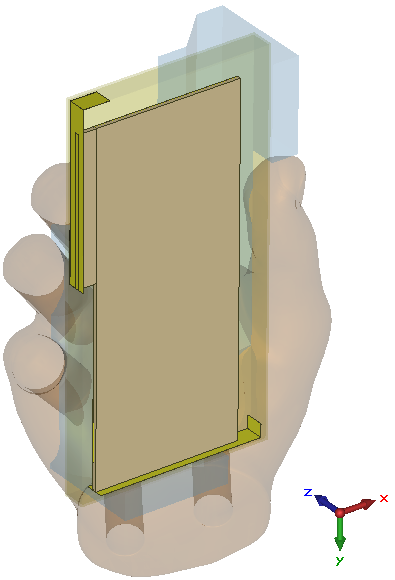
\includegraphics[width=\linewidth,height=4cm,keepaspectratio]{img/tech_sol/trianglefeed/read_mode/3d.PNG}
        \caption{Read mode.}
    \end{subfigure}
    \begin{subfigure}[b]{0.24\linewidth}
        \centering
        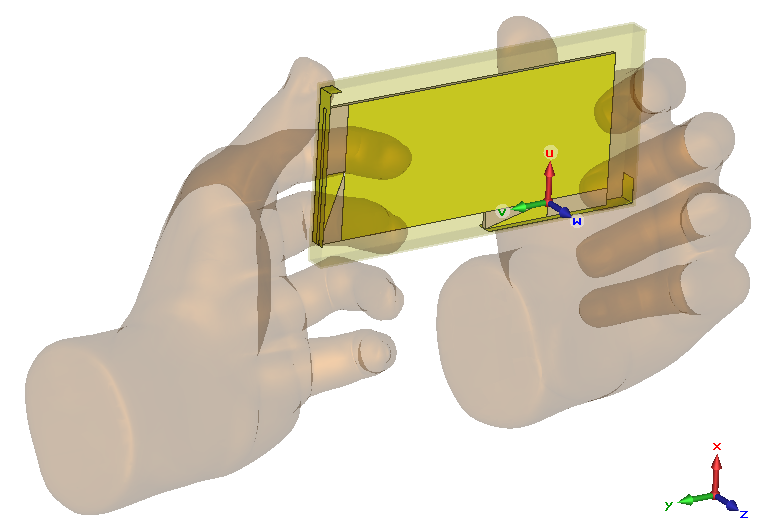
\includegraphics[width=\linewidth,height=4cm,keepaspectratio]{img/tech_sol/trianglefeed/play_mode/3d.PNG}
        \caption{Play mode.}
    \end{subfigure}
    \begin{subfigure}[b]{0.24\linewidth}
        \centering
        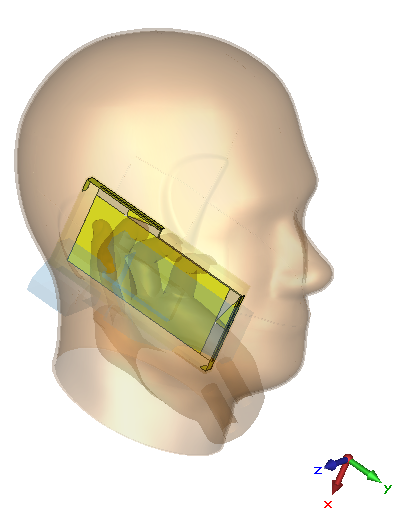
\includegraphics[width=\linewidth,height=4cm,keepaspectratio]{img/tech_sol/trianglefeed/talk_mode/3d.PNG}
        \caption{Talk mode.}
    \end{subfigure}
    \begin{subfigure}[b]{0.24\linewidth}
        \centering
        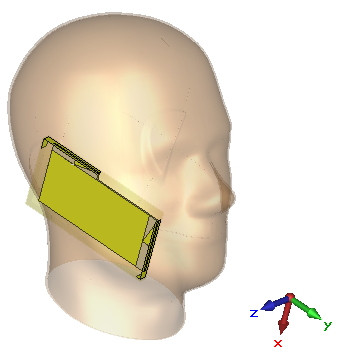
\includegraphics[width=\linewidth,height=4cm,keepaspectratio]{img/tech_sol/trianglefeed/sar/3d.PNG}
        \caption{SAR.}
    \end{subfigure}
    \caption{Antenna position for each user effect simulation.}
    \label{fig:triang_positions}
\end{figure}

\FloatBarrier
\subsection{Read Mode}

\begin{figure}[htbp]
    \centering
    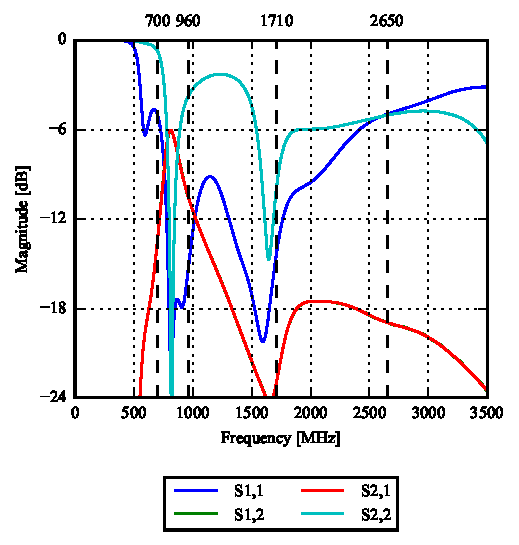
\includegraphics{img/tech_sol/trianglefeed/read_mode/sparams.pdf}
    \caption{Triangular feed antenna in read mode. S-parameters with both tuning capacitors fixed at \SI{0.3}{pF}.}
    \label{fig:triang_sparam_read}
\end{figure}

\begin{table}[htbp]
    \centering
    \begin{tabular}{|l|l|r|r|r|}
        \hline
        Antenna & Band & Start [MHz] & Stop [MHz] & Bandwidth [MHz] \\
        \hline
        Top     & Low  & 570         & 2583       & 2013 \\
        Side    & Low  & 779         & 891        & 112  \\
        \hline
        Top     & High & 570         & 2583       & 2013 \\
        Side    & High & 1506        & 2623       & 1117 \\
        \hline
    \end{tabular}
    \caption{Triangle feed antenna in read mode. Maximum bandwidth obtained in the low and high band for the top and the side antenna, respectively. It is seen that, for the low capacitor settings on the top antenna, both the low and high band are covered at the same time.}
    \label{tab:bw_sol2read}
\end{table}

\begin{figure}[htbp]
   \begin{subfigure}[b]{0.49\linewidth}
        \centering
        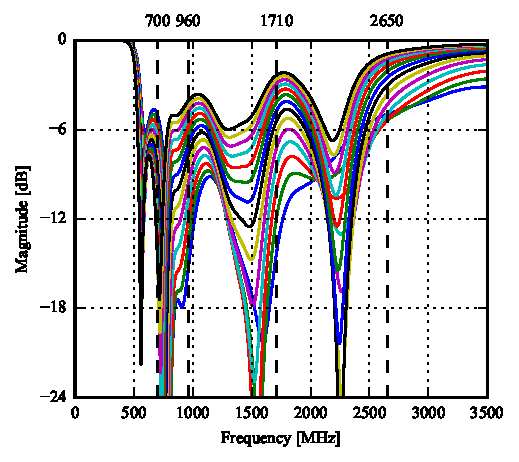
\includegraphics{img/tech_sol/trianglefeed/read_mode/Csh1s11.pdf}
        \caption{$S_{11}$, sweeping $C_1$ and fixing $C_2$.}
    \end{subfigure}
    \hfill
    \begin{subfigure}[b]{0.49\linewidth}
        \centering
        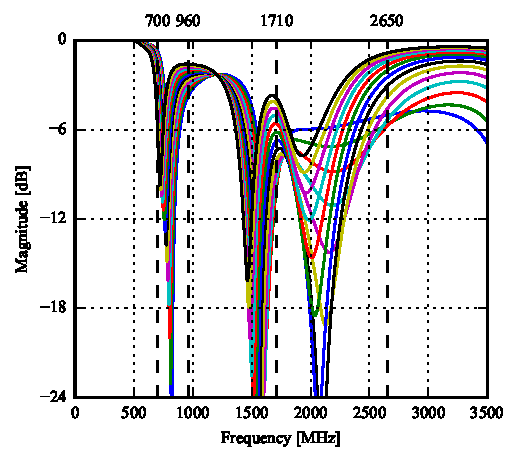
\includegraphics{img/tech_sol/trianglefeed/read_mode/Csh2s22.pdf}
        \caption{$S_{22}$, sweeping $C_1$ and fixing $C_2$.}
    \end{subfigure}
    \\
    \begin{subfigure}[b]{0.49\linewidth}
        \centering
        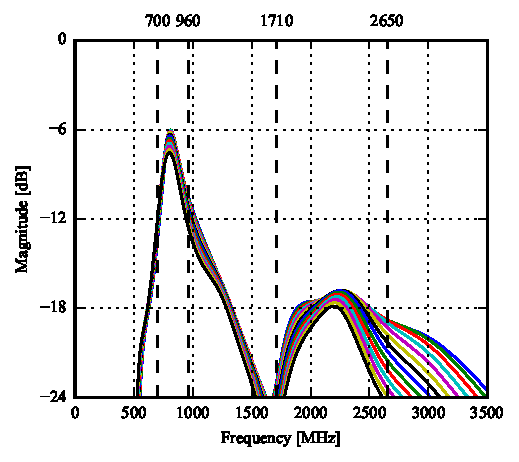
\includegraphics{img/tech_sol/trianglefeed/read_mode/Csh1s21.pdf}
        \caption{$S_{21}$, sweeping $C_1$ and fixing $C_2$.}
    \end{subfigure}
    \hfill
    \begin{subfigure}[b]{0.49\linewidth}
        \centering
        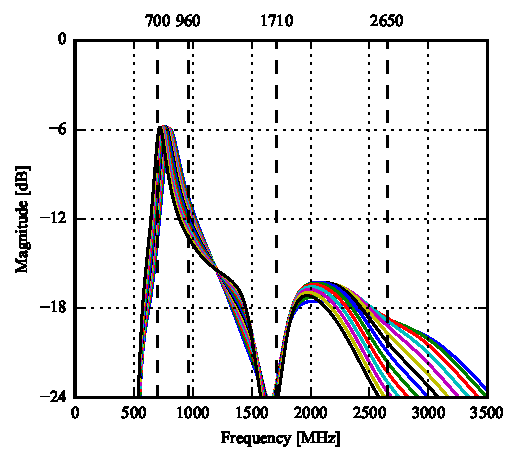
\includegraphics{img/tech_sol/trianglefeed/read_mode/Csh2s21.pdf}
        \caption{$S_{21}$, sweeping $C_2$ and fixing $C_1$.}
    \end{subfigure}
    \caption{Triangle feed antenna in read mode. Parameter sweep for tuning the shunt capacitor of each antenna, $C_1$ and $C_2$ for port 1 and 2, respectively. Port 1 is the top antenna and port 2 is the side antenna.}
    \label{fig:tiang_sparam_sweep_read}
\end{figure}


\FloatBarrier
\subsection{Play Mode}

\begin{figure}[htbp]
    \centering
    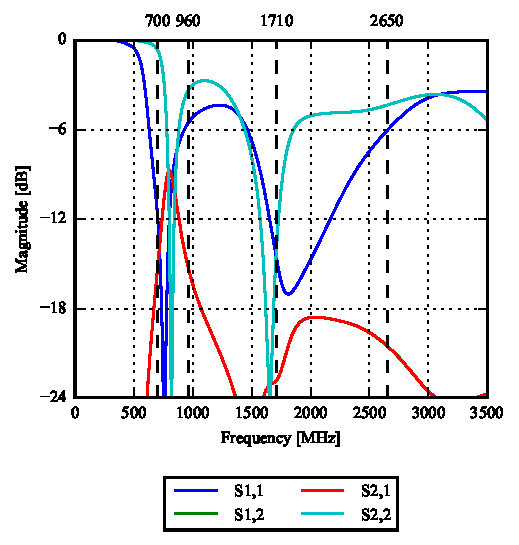
\includegraphics{img/tech_sol/trianglefeed/play_mode/sparams.pdf}
    \caption{Triangular feed antenna in play mode. S-parameters with both tuning capacitors fixed at \SI{0.3}{pF}.}
    \label{fig:triang_sparam_play}
\end{figure}

\begin{table}[htbp]
    \centering
    \begin{tabular}{|l|l|r|r|r|}
        \hline
        Antenna & Band & Start [MHz] & Stop [MHz] & Bandwidth [MHz] \\
        \hline
        Top     & Low  & 629         & 928        & 299  \\
        Side    & Low  & 780         & 881        & 101  \\
        \hline
        Top     & High & 1379        & 2703       & 1324 \\
        Side    & High & 1388        & 2559       & 1171 \\
        \hline
    \end{tabular}
    \caption{Triangle feed antenna in play mode. Maximum bandwidth obtained in the low and high band for the top and the side antenna, respectively. The bandwidth for the side antennas high band is ignoring the slight rise above \SI{-6}{dB} in the middle of the high band.}
    \label{tab:bw_sol2play}
\end{table}

\begin{figure}[htbp]
   \begin{subfigure}[b]{0.49\linewidth}
        \centering
        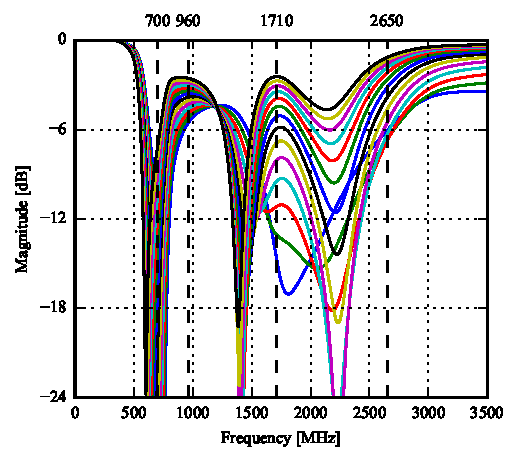
\includegraphics{img/tech_sol/trianglefeed/play_mode/Csh1s11.pdf}
        \caption{$S_{11}$, sweeping $C_1$ and fixing $C_2$.}
    \end{subfigure}
    \hfill
    \begin{subfigure}[b]{0.49\linewidth}
        \centering
        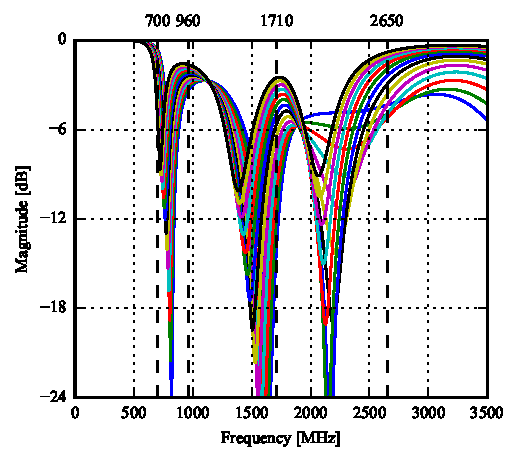
\includegraphics{img/tech_sol/trianglefeed/play_mode/Csh2s22.pdf}
        \caption{$S_{22}$, sweeping $C_1$ and fixing $C_2$.}
    \end{subfigure}
    \\
    \begin{subfigure}[b]{0.49\linewidth}
        \centering
        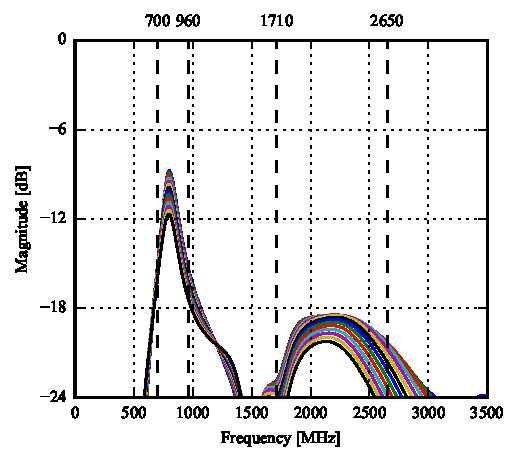
\includegraphics{img/tech_sol/trianglefeed/play_mode/Csh1s21.pdf}
        \caption{$S_{21}$, sweeping $C_1$ and fixing $C_2$.}
    \end{subfigure}
    \hfill
    \begin{subfigure}[b]{0.49\linewidth}
        \centering
        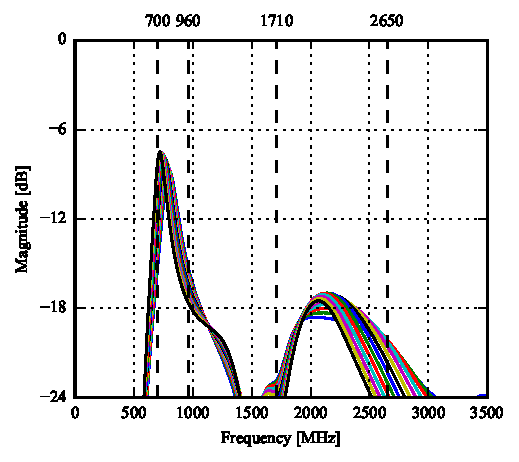
\includegraphics{img/tech_sol/trianglefeed/play_mode/Csh2s21.pdf}
        \caption{$S_{21}$, sweeping $C_2$ and fixing $C_1$.}
    \end{subfigure}
    \caption{Triangle feed antenna in play mode. Parameter sweep for tuning the shunt capacitor of each antenna, $C_1$ and $C_2$ for port 1 and 2, respectively. Port 1 is the top antenna and port 2 is the side antenna.}
    \label{fig:tiang_sparam_sweep_play}
\end{figure}

\FloatBarrier
\subsection{Talk Mode}

\begin{figure}[htbp]
    \centering
    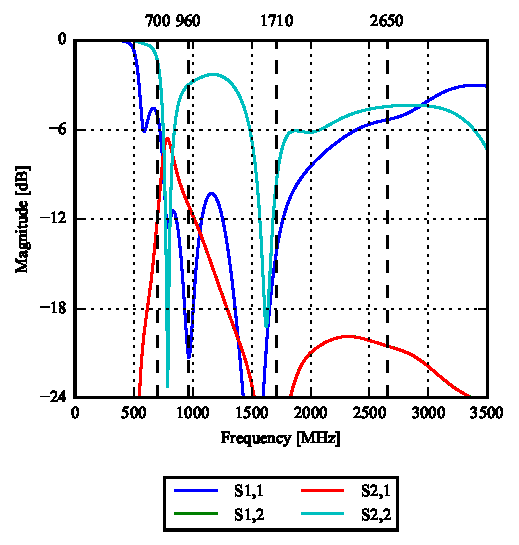
\includegraphics{img/tech_sol/trianglefeed/talk_mode/sparams.pdf}
    \caption{Triangular feed antenna in talk mode. S-parameters with both tuning capacitors fixed at \SI{0.3}{pF}.}
    \label{fig:triang_sparam_talk}
\end{figure}

\begin{table}[htbp]
    \centering
    \begin{tabular}{|l|l|r|r|r|}
        \hline
        Antenna & Band & Start [MHz] & Stop [MHz] & Bandwidth [MHz] \\
        \hline
        Top     & Low  & 701         & 2597       & 1896 \\
        Side    & Low  & 749         & 844        & 95   \\
        \hline
        Top     & High & 701         & 2597       & 1896 \\
        Side    & High & 1439        & 2516       & 1077 \\
        \hline
    \end{tabular}
    \caption{Triangle feed antenna in talk mode. Maximum bandwidth obtained in the low and high band for the top and the side antenna, respectively. It is, again, seen that both the low and high band are covered at the same time for the top antenna.}
    \label{tab:bw_sol2talk}
\end{table}

\begin{figure}[htbp]
   \begin{subfigure}[b]{0.49\linewidth}
        \centering
        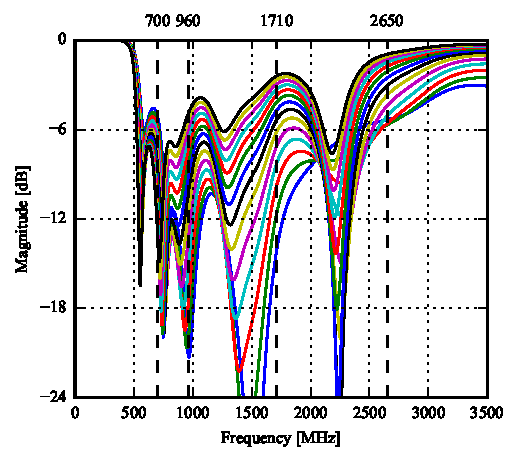
\includegraphics{img/tech_sol/trianglefeed/talk_mode/Csh1s11.pdf}
        \caption{$S_{11}$, sweeping $C_1$ and fixing $C_2$.}
    \end{subfigure}
    \hfill
    \begin{subfigure}[b]{0.49\linewidth}
        \centering
        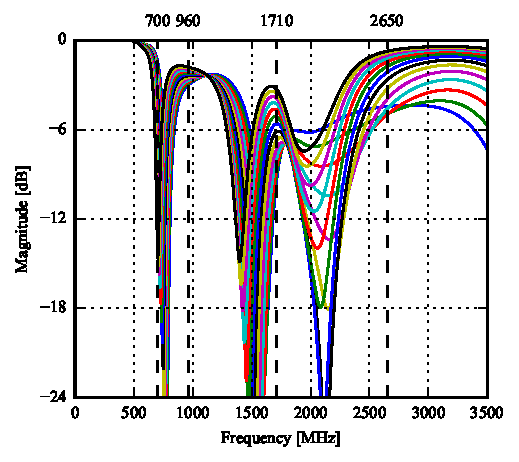
\includegraphics{img/tech_sol/trianglefeed/talk_mode/Csh2s22.pdf}
        \caption{$S_{22}$, sweeping $C_1$ and fixing $C_2$.}
    \end{subfigure}
    \\
    \begin{subfigure}[b]{0.49\linewidth}
        \centering
        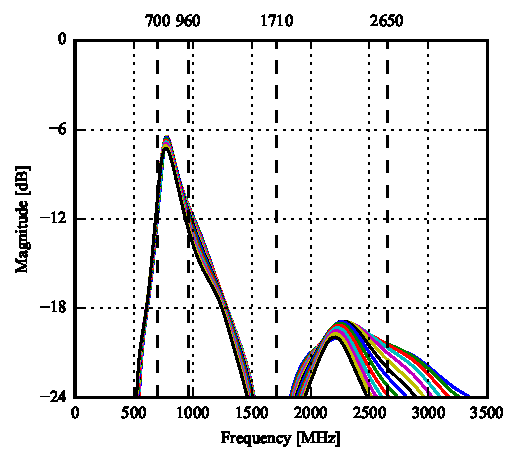
\includegraphics{img/tech_sol/trianglefeed/talk_mode/Csh1s21.pdf}
        \caption{$S_{21}$, sweeping $C_1$ and fixing $C_2$.}
    \end{subfigure}
    \hfill
    \begin{subfigure}[b]{0.49\linewidth}
        \centering
        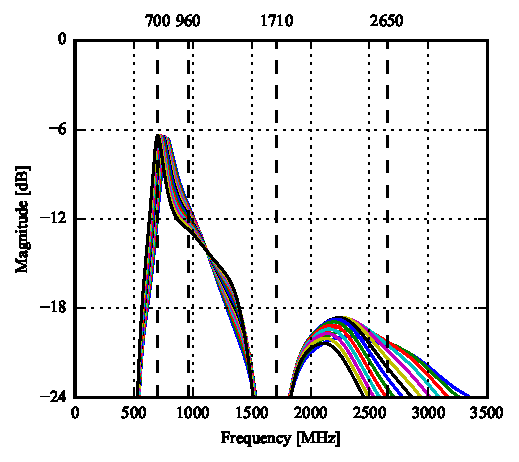
\includegraphics{img/tech_sol/trianglefeed/talk_mode/Csh2s21.pdf}
        \caption{$S_{21}$, sweeping $C_2$ and fixing $C_1$.}
    \end{subfigure}
    \caption{Triangle feed antenna in talk mode. Parameter sweep for tuning the shunt capacitor of each antenna, $C_1$ and $C_2$ for port 1 and 2, respectively. Port 1 is the top antenna and port 2 is the side antenna.}
    \label{fig:tiang_sparam_sweep_talk}
\end{figure}

\FloatBarrier
\subsection{SAR}
The result from the SAR simulation is shown in Figure~\ref{fig:triang_sar_sim}. It is seen, that the maximum SAR is greater than the required maximum of \SI{2}{kg/W}.

\begin{figure}[htbp]
    \centering
    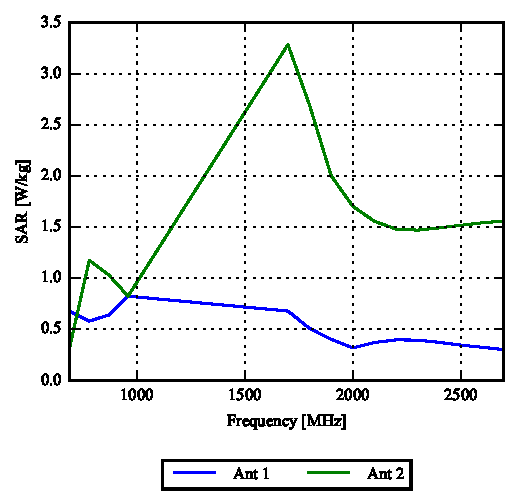
\includegraphics{img/tech_sol/trianglefeed/sar/sar.pdf}
    \caption{SAR simulation of the triangle feed antenna. \fixme{Insert SAR for antenna 2!}}
    \label{fig:triang_sar_sim}
\end{figure}


